\chapter{Viscoelastic Predictions}
%The ultrasound method \cite{Foiret2014} enables the simultaneous measurement of cortical thickness and tissue elastic properties where previous techniques such as DXA (the \textit{de facto} method) could archieve.
As explained before, factors of risk fracture such as thickness, porosity and particular quality elements of the extracellular matrix, define the bone quality assessed by DXA techniques and BMD values. The QUS method \textit{Minonzio and Foiret et al.} \cite{Foiret2014}, \cite{Minonzio2018} of axial transmission technique simulated in the chapter before, is based on recording from the guided-wave propagation over the media, where damping factors naturally affect the signal. This relates to a viscoelastic behavior of the cortical bone arising mainly from the presence of collagen fibers, specifically treated with Resonant Ultrasound Spectroscopy (RUS) techniques. Thus, it becomes natural to study the correspondence between such damping elements and their preponderance on the resulting homogenized coefficients by the two-scale homogenization theory.

Describing the damping effects on cortical bone is not new, \textit{Bernard} \textit{et al. }\cite{Bernard2015} studied a viscoelastic-type behavior on a frequency domain, in which he modelled the elastic tensor $C^*_{ij}$ with damping effect described by the formulas:
\begin{equation*}
C^*_{ij} = C_{ij} + i C_{ij}^{'} = C_{ij} (1+ iQ_{ij}^{-1}) \quad i,j = 1,\dots, 6
\end{equation*}
where the $Q^{-1}_{ij}$ are defined as ratios of the imaginary part ($C_{ij}'$) to the real part ($C_{ij}$), denoting the so-called quality factors.

In this section, I shall reformulate such quality factors following the two-scale homogenization formalism, recovering the homogenized coefficients in the elastic case at different porosity levels and particularly obtaining prediction for the quality factors at some interval. Using up-to-date references, such coefficients are yet to be validated since there isn't enough experimental literature to confirm nor further validate the predictions.

\section{Formalization of Q-factors}
The quality factors $Q_{ij}$ proposed by \textit{Bernard} in experimental fashion, provide an interesting formalization of the ratio between the real and imaginary constitutive coefficients of a full viscoelastic mechanical description of the bone, moreover it gives us a comparison using the existent literature and experimental results.

In the following, it's described the so-called Q-factors by means of the two-scale homogenization theory, derived from a \textit{Kelvin-Voigt} viscoelastic formulation of bone in frequency domain. More specifically, it's defined the mechanical behavior of bone as a multiphase viscoelastic material composed of two-phases with cell unit in the form $\mathbf{Y} = Y_{m} \cup Y_{f}$ being each the matrix and fluid parts respectively.
For the bone matrix, we associate an elastic behavior defined by the elastic coefficients:
\begin{equation*}
    C_{ijkl}(\mathbf{y}) = C_{ijkl}^m \mathbb{I}_{Y_m}(\mathbf{y}) + C_{ijkl}^f \mathbb{I}_{Y_f}(\mathbf{y})
\end{equation*}
while the porosity is modeled with a viscous contribution, associated to coefficients in the form:
\begin{equation*}
    D_{ijkl}(\mathbf{y}) =  D_{ijkl}^m \mathbb{I}_{Y_m}(\mathbf{y}) + D_{ijkl}^f \mathbb{I}_{Y_f}(\mathbf{y})
\end{equation*}
Moreover, the relations between both behaviors are expressed with attenuation specified by parameters $\epsilon^{(m)}, \epsilon^{(f)} >0$ associated to the bone matrix and mesostructure respectively. Explicitly, it's assumed:
\begin{equation*}
    D_{ijkl}^m(\mathbf{y}) = \alpha^{m} C_{ijkl}^m(\mathbf{y}) , \quad D_{ijkl}^f (\mathbf{y}) = \alpha^{f} C_{ijkl}^f(\mathbf{y})
\end{equation*}


\begin{rem}
By assuming this kind of relation, the objective is to obtain a viscoelastic model in which the viscous part is modelled by a linear attenuation of the elastic one, so that the overall behavior is of transverse isotropic type defined by pair of parameters $(\alpha^m, \alpha^f)$ that mimic closely the experimental behavior of cortical bone.
\end{rem}

\subsection{Workflow Description}
Given the requirements of a viscous-like behavior, in time domain it's considered a model of \textit{Kelvin-Voigt} type with mixed boundary conditions, described in the form:
\begin{equation*}
    \left \{
    \begin{array}{cc}
        \rho^{\epsilon}\partial_{tt}u^{\epsilon} - \nabla \cdot \sigma(u^{\epsilon}, \partial_t u^{\epsilon}) = \mathbf{0} & \text{ in } (0,T) \times \Omega\\
        \sigma^{\epsilon}(u^{\epsilon},\partial_t u^{\epsilon})  = \mathbf{C}:\mathbf{e}(u^{\epsilon}) + \mathbf{D}:\mathbf{e}(\partial_t u^{\epsilon}) & \text{ in } (0,T) \times \Omega\\
        \sigma^{\epsilon}(u^{\epsilon}, \partial_t u^{\epsilon})\cdot n = \mathbf{F} & \text{ on } (0,T) \times \Gamma_N\\ 
        u^{\epsilon} = \mathbf{0} & \text{ on } (0,T) \times \Gamma_D
    \end{array}
    \right .
    \label{ViscoElasticModel}
\end{equation*}
\begin{rem}
In the above and the next developments, we assume resting initial conditions, i.e., $\partial_t u^{\epsilon} = u^{\epsilon} = \mathbf{0}$, not written explicitly in the models and deduction.
\end{rem}
Existence results can be derived similarly to the elastic case proposed before, by applying spectral decomposition on both: the elastic and viscoelastic operators. Similar mathematical description of viscous models are given by \cite{Abdessamad2009}, \cite{Boughammoura2013} on homogeneous \textit{Dirichlet} boundary condition cases.

The interest is regarded to the frequency-domain, thus applying \textit{Fourier} transform defined at frequency $\omega \in \mathbb{R}$ with base $\{e^{i\omega t}\}_{\omega}$, it's obtained the redefined problem in Fourier domain as follows:
\begin{equation*}
    \left \{
    \begin{array}{cc}
        -\omega^2 \rho^{\epsilon} \hat{u}^{\epsilon} - \nabla \cdot \hat{\sigma}_{\epsilon,\omega}(\hat{u}^{\epsilon}) = \mathbf{0} & \text{ in } \Omega  \\
        \hat{\sigma}_{\epsilon,\omega} (\hat{u}^{\epsilon}) = (\mathbf{C} + i\omega \mathbf{D}):\mathbf{e}(\hat{u}^{\epsilon}) & \text{ in } \Omega \\
        \hat{\sigma}_{\epsilon,\omega} (\hat{u}^{\epsilon}) \cdot n = \hat{\mathbf{F}}(\omega) & \text{ on } \Gamma_N \\
        \hat{u}^{\epsilon} = \mathbf{0} & \text{ on } \Gamma_D
    \end{array}
    \right .
\end{equation*}
such that at $\omega = 0$ we have $\hat{u}^{\epsilon}=\mathbf{0}$ at $\Omega$. In particular, for easiness of exposure, it has been omitted dependencies on the frequency for the multiscale solution $u^{\epsilon}$.\\

Now, by the homogenization heuristic using the two-scale asymptotic method, it follows the effective (macroscopic) model defined at frequency $\omega$ in the form:
\begin{equation*}
    \left \{
    \begin{array}{cc}
        -\omega^2 \rho^{0} \hat{u}^0 - \nabla \cdot \hat{\sigma}^0(\hat{u}^0)  = \mathbf{0} & \text{ in } \Omega \\
        \hat{\sigma}^{0} (\hat{u}^0)  = (\mathbf{C} + i\omega \mathbf{D})^{hom}:\mathbf{e}(\hat{u}^0) & \text{ in } \Omega \\
        \hat{\sigma}^{0} (\hat{u}^0) \cdot n = \hat{\mathbf{F}}(\omega) & \text{ on } \Gamma_N \\
        \hat{u}^0 = \mathbf{0} & \text{ on } \Gamma_D
    \end{array}
    \right .
\end{equation*}

In particular, the homogenized coefficients, are defined by the cell problem solutions $N^{rs} \in \mathbf{H}^1_{\#}(\mathbf{Y}, \mathbb{C})$, described for each $r,s \in \{1,2,3\}$ in the form
\begin{equation*}
    \left \{
    \begin{array}{cc}
         \partial_{y_j} \big[ \big( C_{ijkl} + i\omega D_{ijkl} \big) \mathbf{e}_{kl}(N^{rs}) \big] &= - \partial_{y_j} \big[ C_{ijkl} + i\omega D_{ijkl} \big] \quad \forall y \in \mathbf{Y} \\
        \big \langle C_{ijkl} + p D_{ijkl} \big \rangle_{\mathbf{Y}}  = 0 & 
    \end{array}
    \right.
\end{equation*}
Since the cell problems must be valid for each $\omega \in \mathbb{R}$ and for each $\mathbf{y} \in \mathbf{Y}$, a natural procedure would be to decouple the cell PDE problems thus being possible the definition of viscosity-elasticity ratios, i.e. an expression to the so-called Q-factors.

The decoupling is then defined by considering the separation between real and imaginary parts associated to the cell solutions, i.e., by considering the following decomposition
\begin{equation*}
    N^{rs}(\mathbf{y}) = \mathbf{N}_R^{rs}(\mathbf{y}) + i\mathbf{N}_I^{rs}(\mathbf{y})
\end{equation*}
being now the vectors functions $\mathbf{N}_R^{rs}, \mathbf{N}_I^{rs}$ in $\mathbf{H}^1_{\#}(\mathbf{Y},\mathbb{R})$ solving the following PDE coupled system for each real and imaginary solution parts in the form:
\begin{equation*}
    \left \{
    \begin{array}{cc}
        \partial_{y_j} \big[ C_{ijkl} \mathbf{e}_{kl}(\mathbf{N}^{rs}_R) -\omega D_{ijkl} \mathbf{e}_{kl}(\mathbf{N}^{rs}_I) \big] = - \partial_{y_j} \big[ C_{ijrs} \big] & \forall \mathbf{y} \in \mathbf{Y} \\
        \partial_{y_j} \big[ C_{ijkl} \mathbf{e}_{kl}(\mathbf{N}^{rs}_I) +\omega D_{ijkl} \mathbf{e}_{kl}(\mathbf{N}^{rs}_R) \big] = - \partial_{y_j} \big[ \omega D_{ijrs} \big] & \forall \mathbf{y} \in \mathbf{Y} \\
        \big \langle \mathbf{N}^{rs}_R \big \rangle_{\mathbf{Y}},\big \langle \mathbf{N}^{rs}_I \big \rangle_{\mathbf{Y}} = \mathbf{0}  &
    \end{array}
    \right.
\end{equation*}
\begin{rem}
Note in particular that for the above cell problems, we existence and uniqueness of a weak solution is guaranteed since the problem can be rewritten as a fully elliptic operator, being the solution unique by applying a normalization condition of mean equal $\mathbf{0}$ type.
\end{rem}
With the solution to the cell problem, we can then define the homogenized coefficients associated to the elastic and viscous part by recalling first:
\begin{equation*}
    \hat{\sigma}_{ij}^0 (\hat{u}^0,\omega) = R_{ijkl}^{hom} (\omega) \mathbf{e}_{kl}(\hat{u}^0)
\end{equation*}
being the homogenized tensor
\begin{equation*}
    R^{hom}_{ijrs}= \big \langle  C_{ijrs} + i\omega D_{ijrs} + \big( C_{ijkl} + i \omega D_{ijkl} \mathbf{e}_{kl}(\mathbf{N}^{rs}) \big) \big \rangle  
\end{equation*}
so that, using the decomposition of $N^{rs}$ it follows the full homogenized expression, described in (\ref{ViscoElasticDecom}) decomposed in real and imaginary parts characterizing the elastic and viscous contribution respectively.
\begin{equation}
    \begin{aligned}
        R^{hom}_{ijrs} &= \big \langle C_{ijrs} + \big( C_{ijkl}\mathbf{e}_{kl}( \mathbf{N}^{rs}_R) -\omega D_{ijkl}\mathbf{e}_{kl}(\mathbf{N}^{rs}_I) \big) \big \rangle \\
        & \, + i \big \langle \omega D_{ijrs} + \big( C_{ijkl} \mathbf{e}_{kl}(\mathbf{N}^{rs}_I) + \omega D_{ijkl}\mathbf{e}_{kl}(\mathbf{N}^{rs}_R) \big) \big \rangle \\
        & := C^{hom}_{ijrs} + \mathbf{i} \omega D^{hom}_{ijrs}
    \end{aligned}
    \label{ViscoElasticDecom}
\end{equation}

In particular, the definition of $Q_{ij}$ factors can be directly rewritten terms of a homogenized formulation, defined directly on the tensor coefficients described by (\ref{Qfactor-Def}). In particular, given the deduction done, the definition of such quality-factors becomes dependent on the frequency which derives from the multiscale \textit{Kelvin-Voigt} mechanical model assumed.
\begin{equation}
    \label{Qfactor-Def}
    Q_{ijrs}^{-1}(\omega) := \frac{D^{hom}_{ijrs}(\omega)}{ C^{hom}_{ijrs}(\omega)}
\end{equation}


\subsection{Nonlinear Decomposition}

An aspect that must be taken into account is the nonlinear effect added from the asymptotic assumption on the solution, expressed in the term $N^{rs}$ at the homogenized coefficients definition that can be explicitly stated from (\ref{Qfactor-Def}).
It's possible to account for that effect by taking a decomposition on the linear part associated to the mean over the coefficient itself and the nonlinear effect produced from the solutions to the cell problems, i.e., from (\ref{Qfactor-Def}) the decomposition in its linear and nonlinear effects its obtained as:
\begin{equation}
    \label{Expansion-Qfactor}
        Q_{ijrs}^{-1} =  \frac{D_{hom}^{(0)}}{C_{hom}^{(0)}} + \frac{1}{C^{(0)}_{hom}\left( C^{(0)}_{hom} + C^{(1)}_{hom} \right)} \big[C^{(0)}_{hom} \big( D^{(0)}_{hom} + D^{(1)}_{hom}\big) - D^{(0)}\big( C^{(0)}_{hom} + C^{(1)}_{hom} \big) \big]
\end{equation}
where its being used the notation for the linear terms in $p \in [0,1]$ (porosity) by:
\begin{equation*}
    C^{(0)}_{hom} = \langle C_{ijrs} \rangle_{\mathbf{Y}} \quad  D^{(0)}_{hom} = \langle D_{ijrs} \rangle_{\mathbf{Y}}
\end{equation*}
and the nonlinear terms with respect to $p \in [0,1]$ associated to the solutions $N^{rs}$ given by:
\begin{equation*}
    \begin{array}{cc}
        C^{(1)}_{hom} =& \langle C_{ijkl}\mathbf{e}_{kl}(N^{rs}_R) - \omega D_{ijkl}\mathbf{e}_{kl}(N^{rs}_I) \rangle_{\mathbf{Y}} \\
        D^{(1)}_{hom} =& \langle \omega^{-1} C_{ijkl}\mathbf{e}_{kl}(N^{rs}_I) + D_{ijkl}\mathbf{e}_{kl}(N^{rs}_R) \rangle_{\mathbf{Y}} 
    \end{array}
\end{equation*}




\section{Predictions}
\begin{rem}
For the 2-dimensional modelling case of transverse isotropic material, the simulated solutions are close enough to \textit{Parnel and Grimal} prediction with their approximation method.
\end{rem}

The explicit dependency on the frequency $\omega$, requires us to consider the frequency range in which the experimental setting take place. In this sense, after adjusting regards experimental data range, viscous factors with transverse isotropic behavior of the type are assumed in the form:
\begin{equation*}
    D^m_{ijkl} (\mathbf{y}) = 5\times10^{-2} C^{m}_{ijkl}(\mathbf{y}), \quad D^f_{ijkl}(\mathbf{y}) = 1 \times 10^{-3} C^{f}_{ijkl}(\mathbf{y})
\end{equation*}

Under such considerations, the figure (\ref{BernardPredictionHomCoeffs}) contains the prediction for the homogenized elastic coefficients and Q-factors associated to a fixed frequency $\omega = 0,5 \, [Mhz]$. It describes the behavior as function of density in the clinical range of interest. The main quality factors describing the axial-related behavior shows predictions comparable to up-to-date literature \cite{Bernard2015}. Moreover, homogenized elasticity coefficients are recovered with predictions regarding results obtained in fully elastic models, therefore describing a generalization. 
In particular, shear-like $C_{55}^{hom}, C_{66}^{hom}$ coefficients describe experimentally measured values validating the simulated model.

\begin{figure}[!h]
	\centering
	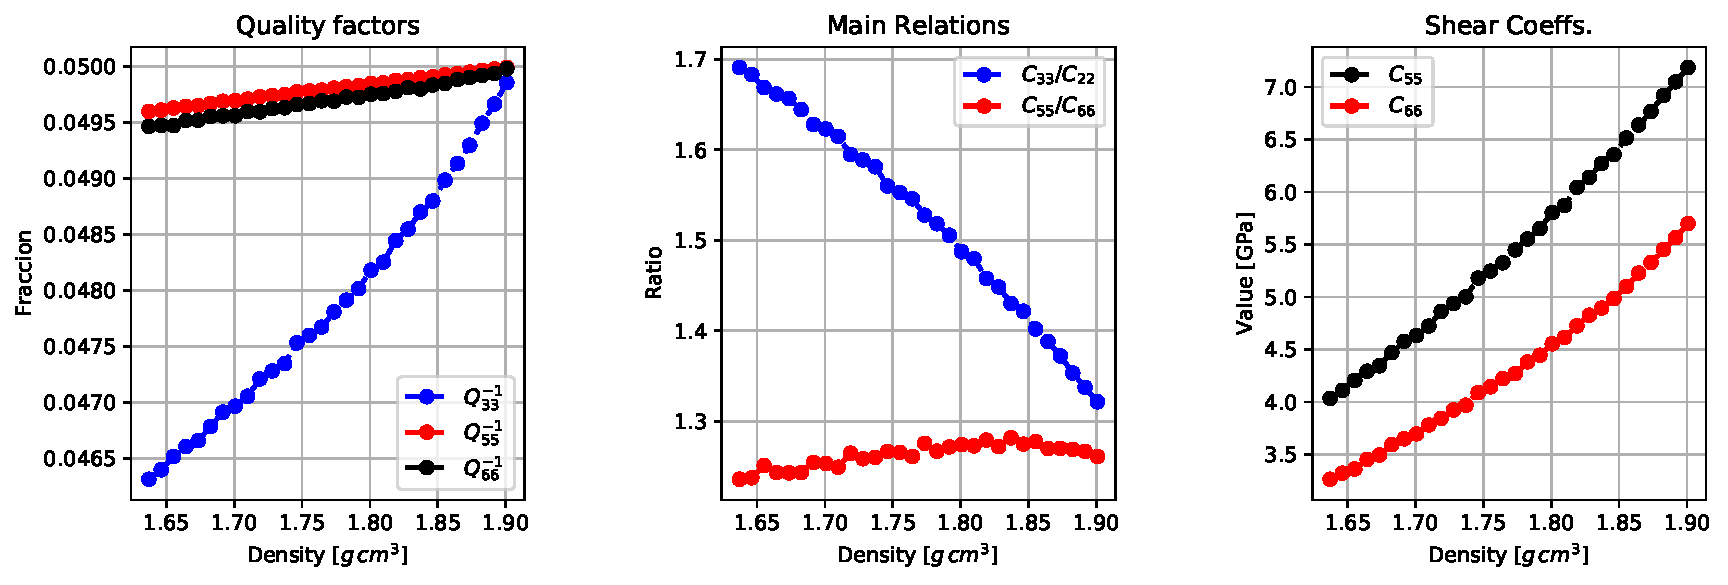
\includegraphics[width=\textwidth]{images/Qfactors/CellProb_QfactorCircular5E-2_Relations.pdf}
	\caption{Predicted Behavior for the Viscoelastic Model. Its shown on the left figure the predicted quality factors for a \textit{Kelvin-Voigt} model; the center figure a prediction of homogenized coefficient ratios, and on the right figure some homogenized shear ratios behaves as in \cite{Bernard2015}.}
	\label{BernardPredictionHomCoeffs}
\end{figure} 

Nevertheless, figure (\ref{BernardPredictionHomCoeffs}) cannot be used to account for the nonlinearity effects which might not be preponderant on the definition of the quality factors. In this setting, the decomposition (\ref{Expansion-Qfactor}) can be used to describe characteristic behavior regarding the linear and nonlinear contribution and therefore, answering the question of dependency on preponderant linear behavior. It shows a clear
direction-dependent strong non-linear preponderance on the overall behavior for the three cases shown implying full cell-problem interactions to describe each factors. In particular, becoming the cell-problems the most relevant effect that describes the mechanical behavior.

\begin{figure}[!h]
	\centering
	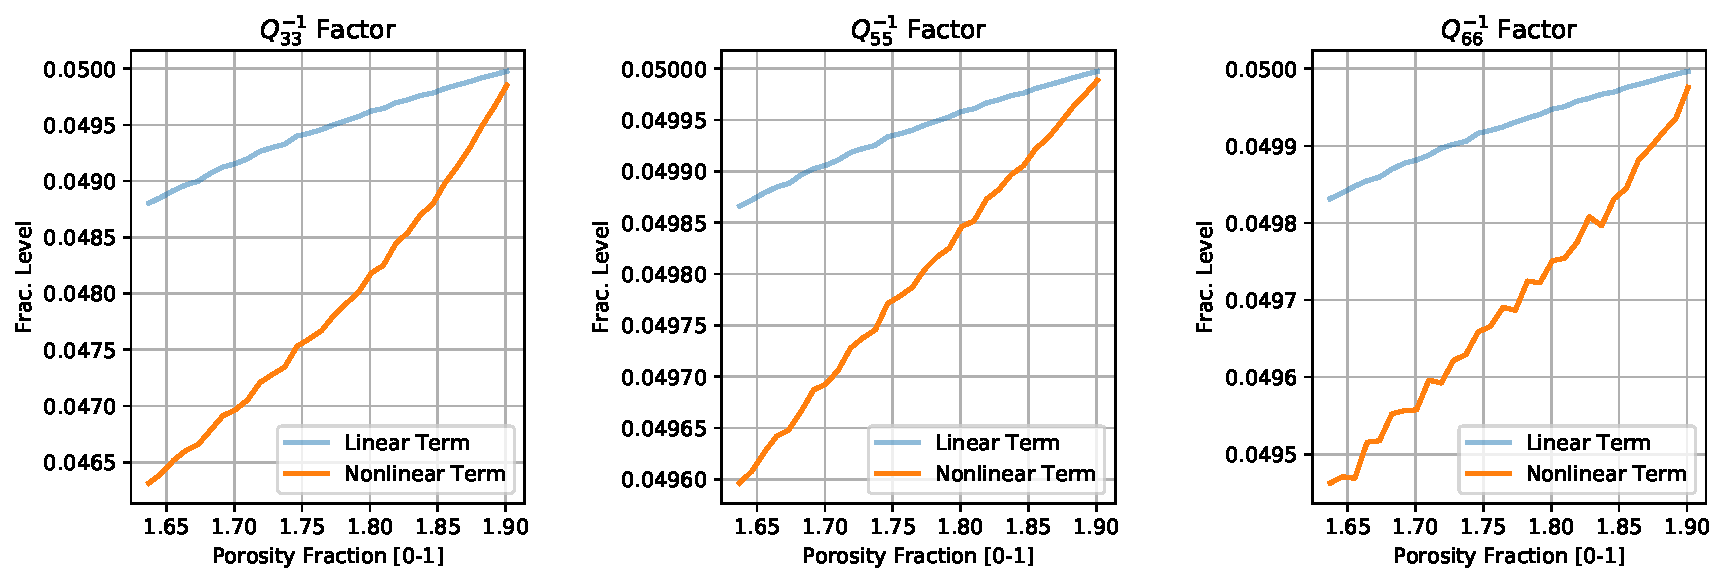
\includegraphics[width=\textwidth]{images/Qfactors/PlotsVisc_Circular2DPart50EPS5-2_Ome05.pdf}
	\caption{The effects from cell-problem solutions is shown for some representative quality factors accounting the linear and non-linear contributions over the range of biomedical interest.}
	\label{QfactorDecomposition}
\end{figure} 

A relevant dependency that must be taken into account from the Q-factors (\ref{Qfactor-Def}) is related to the frequency-dependency. From the experimental setting proposed by \cite{Bernard2015}, such dependency is not taken into account on the viscoelastic operator nor in the quality-factor. 
Studying such dependency, figure (\ref{BernardPrediction-Freq}) describes the obtained factors for different frequency values. They shown a clear in-dependency towards the frequency being used, therefore expressing the assumption proposed by \cite{Bernard2015} in which given the frequency range under consideration, the overall Q-elastic behavior is the same, i.e., equal on the elastic and viscous part of the elastodynamic model given a change of the frequency under simulation.
\begin{figure}[!h]
	\centering
	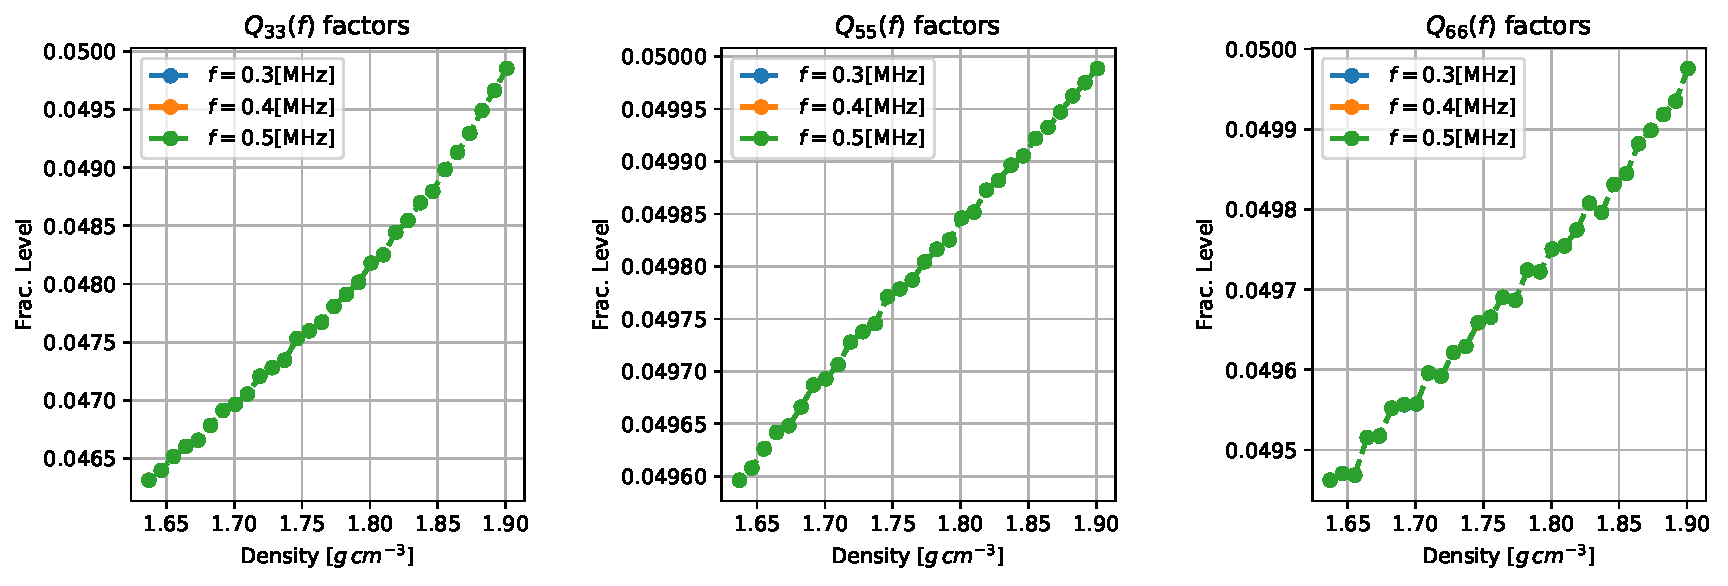
\includegraphics[width=\textwidth]{images/Qfactors/QfactorsFreqsEPS5-2.pdf}
	\caption{Predicted behavior for the viscoelastic model. It is shown in the left figure the predicted quality factors for a \textit{Kelvin-Voigt} model; the center figure a prediction of homogenized coefficient ratios, and in the right figure some homogenized shear ratios behaves as in \cite{Bernard2015} }
	\label{BernardPrediction-Freq}
\end{figure}.






